% !TeX root = ../../../geos_mpm_manual.tex
\section{Background grid}
\label{sec:pfw-background-grid}
\index{background grid}
\index{InternalMesh}
\index{parallel mesh generation}
\index{plane strain!PFW}
\index{refinement!PFW}

PFW writes a GEOS \texttt{InternalMesh} for the background grid.  The main controls are the physical domain bounds \texttt{xmin/xmax}, \texttt{ymin/ymax}, \texttt{zmin/zmax}; the total cell counts \texttt{nI/nJ/nK}; periodic flags \texttt{periodic}; partition counts \texttt{xpar/ypar/zpar}; and particle-density controls \texttt{ppc}, \texttt{ppcx}, \texttt{ppcy}, and \texttt{ppcz}.  The generated mesh uses uniform Cartesian cells and the \texttt{C3D8} element type, even for plane-strain cases, because the MPM solver and particle mesh operate on the GEOS three-dimensional mesh data structures.

\subsection{Parallel grid-generation constraints}
\index{particles per partition}
\index{periodic boundaries!PFW grid}

The practical challenge in parallel PFW generation is to keep each MPI partition balanced while preserving a uniform grid and a simple particle-generation loop.  In typical production inputs, each partition is assigned the same number of cells in each active direction.  This means \texttt{nI}, \texttt{nJ}, and \texttt{nK} should be chosen consistently with \texttt{xpar}, \texttt{ypar}, and \texttt{zpar}.  Periodic and non-periodic directions differ slightly: non-periodic directions include one ghost cell on each side in the total \texttt{InternalMesh} count, whereas periodic directions do not add those two extra cells.  Consequently, PFW computes interior cell counts as
\begin{equation}
  n_x^{\mathrm{int}} =
  \begin{cases}
  N_x, & \text{periodic in }x,\\
  N_x-2, & \text{non-periodic in }x,
  \end{cases}
\end{equation}
and analogously for \(y\) and \(z\), except that plane strain always uses the reduced through-thickness treatment described below.  The interior spacings are then
\begin{equation}
  \Delta x = \frac{x_{\max}-x_{\min}}{n_x^{\mathrm{int}}}, \qquad
  \Delta y = \frac{y_{\max}-y_{\min}}{n_y^{\mathrm{int}}}, \qquad
  \Delta z = \frac{z_{\max}-z_{\min}}{n_z^{\mathrm{int}}}.
\end{equation}

The appropriate number of particles per partition is hardware and model dependent.  A common CPU target is below roughly \(4\times 10^4\) particles per MPI partition for interactive development and moderate material complexity.  On GPU-enabled workflows, substantially larger partitions can be practical; values approaching \(10^6\) particles per partition may be usable for simple kernels and sufficiently large devices.  These are operational guidelines rather than solver limits: constitutive cost, contact fields, neighbor lists, output variables, and available memory can change the useful range by orders of magnitude.

\subsection{Common \texttt{cpp}--\texttt{refine}--\texttt{ppc} pattern}
\index{cells per partition}
\index{cpp}
\index{ppc}

Most suite and example inputs use a small set of derived variables rather than entering every mesh count directly.  The pattern is
\begin{align}
  \texttt{cpp} &= \text{cells per partition in a coordinate direction},\\
  \texttt{refine} &= \text{integer or real resolution multiplier},\\
  \texttt{xpar} &= \max(N_x^{\mathrm{pbc}},\, \mathrm{round}(\texttt{refine}\,\texttt{xpar0})),\\
  \texttt{nI} &= \texttt{xpar}\,\texttt{cpp},
\end{align}
with analogous definitions in \(y\) and \(z\).  Here \(N_x^{\mathrm{pbc}}\) is usually 3 in a periodic direction and 1 otherwise, so that periodic directions have enough partitions for periodic neighbor communication and representative partitioning.  The particle density is then set with \texttt{ppc} or direction-specific values.  With \texttt{ppc=2}, a full three-dimensional cell initially contains \(2^3=8\) candidate particle points before geometry filtering, while a plane-strain cell contains one through-thickness layer and \(2^2=4\) in-plane candidate points.

\begin{figure}[htbp]
  \centering
  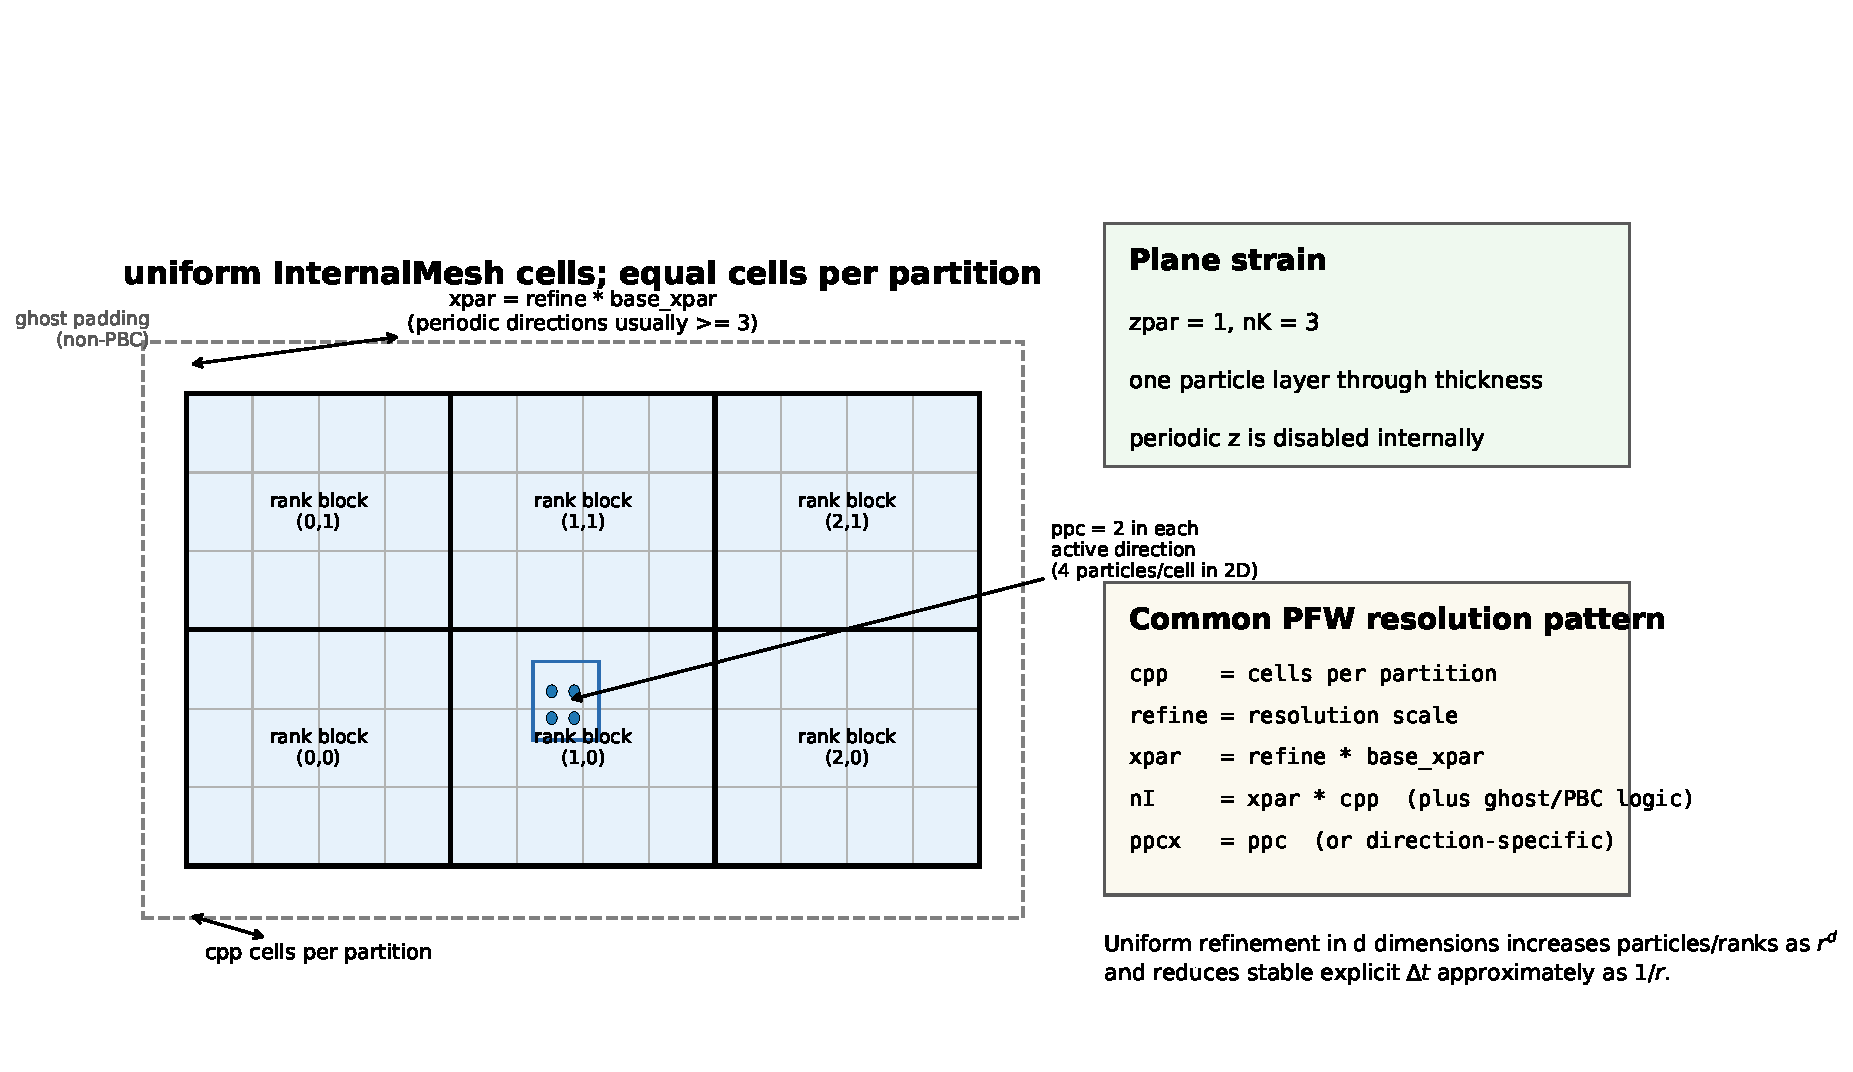
\includegraphics[width=0.92\linewidth]{figures/pfw_grid_partition_schematic.pdf}
  \caption{Typical PFW resolution pattern.  Users select a cells-per-partition count \texttt{cpp}, scale the number of partitions with \texttt{refine}, and choose particles per cell with \texttt{ppc}.  The resulting \texttt{InternalMesh} cells are uniform; non-periodic directions include ghost-cell corrections, while periodic directions generally require at least three partitions in production examples.}
  \label{fig:pfw-grid-partition-schematic}
\end{figure}

A representative input fragment is
\begin{lstlisting}[language=Python,caption={Resolution variables used to populate PFW mesh controls.}]
refine = 3
cpp = 12
base = [1, 1, 1]
pbc_min = [3 if p else 1 for p in pfw["periodic"]]

pfw["xpar"] = max(pbc_min[0], int(round(refine*base[0])))
pfw["ypar"] = max(pbc_min[1], int(round(refine*base[1])))
pfw["zpar"] = max(pbc_min[2], int(round(refine*base[2])))
pfw["nI"] = pfw["xpar"] * cpp
pfw["nJ"] = pfw["ypar"] * cpp
pfw["nK"] = pfw["zpar"] * cpp
pfw["ppc"] = 2
pfw["mCores"] = pfw["xpar"] * pfw["ypar"] * pfw["zpar"]
\end{lstlisting}

\subsection{Plane-strain meshes}
\index{plane strain!mesh}

Plane-strain cases are represented with a three-dimensional GEOS mesh but a reduced particle layer.  The current PFW checks
\begin{equation}
  \texttt{planeStrain}=1 \quad \Rightarrow \quad \texttt{zpar}=1, \qquad \texttt{nK}=3.
\end{equation}
PFW then treats the through-thickness direction as one active interior cell plus ghost padding, creates a single layer of particles through thickness, sets through-thickness particle velocities to zero, and passes \texttt{planeStrain} to the solver.  In-plane controls \texttt{ppcx} and \texttt{ppcy} still set the in-plane particle density; \texttt{ppcz} does not create multiple through-thickness layers in a plane-strain run.  The generated GEOS XML also disables periodicity in the suppressed \(z\) direction when \texttt{planeStrain}=1.

This representation keeps the same particle-file and mesh infrastructure as three-dimensional calculations while reducing the particle count and enforcing the intended kinematics.  Users should still choose a physical \(z\)-extent consistent with the constitutive model and any diagnostic interpretation of force, stress, or reaction quantities.

\subsection{Refinement and cost scaling}
\index{time step!refinement}
\index{CFL condition}
\index{cost scaling}

For explicit MPM, the stable time step scales with the cell size through the CFL condition.  If a fixed physical domain is refined by a factor \(r\) in each active direction, then \(\Delta x\sim r^{-1}\) and the number of steps required to reach a fixed physical time grows approximately as \(r\).  With fixed \texttt{ppc}, the particle count grows as \(r^d\), where \(d=2\) for plane-strain or other effectively two-dimensional calculations and \(d=3\) for full three-dimensional calculations.  The total explicit work to reach a fixed time therefore scales roughly as
\begin{equation}
  W(r) \propto r^{d+1},
\end{equation}
ignoring changes in contact, neighbor-list, constitutive, and communication overheads.  Thus a two-dimensional refinement sequence typically grows like \(r^3\) in total core work, and a three-dimensional sequence like \(r^4\).  If \texttt{cpp} is held fixed while \texttt{refine} increases the number of partitions, the per-rank particle count can remain approximately constant, but the number of time steps still grows as \(r\) and the total number of ranks grows as \(r^d\).  This is why PFW examples tend to expose \texttt{refine}, \texttt{cpp}, and \texttt{ppc} explicitly: the variables make accuracy, memory, and run-time tradeoffs visible in the input file.
